\begin{figure*}
    \centering
    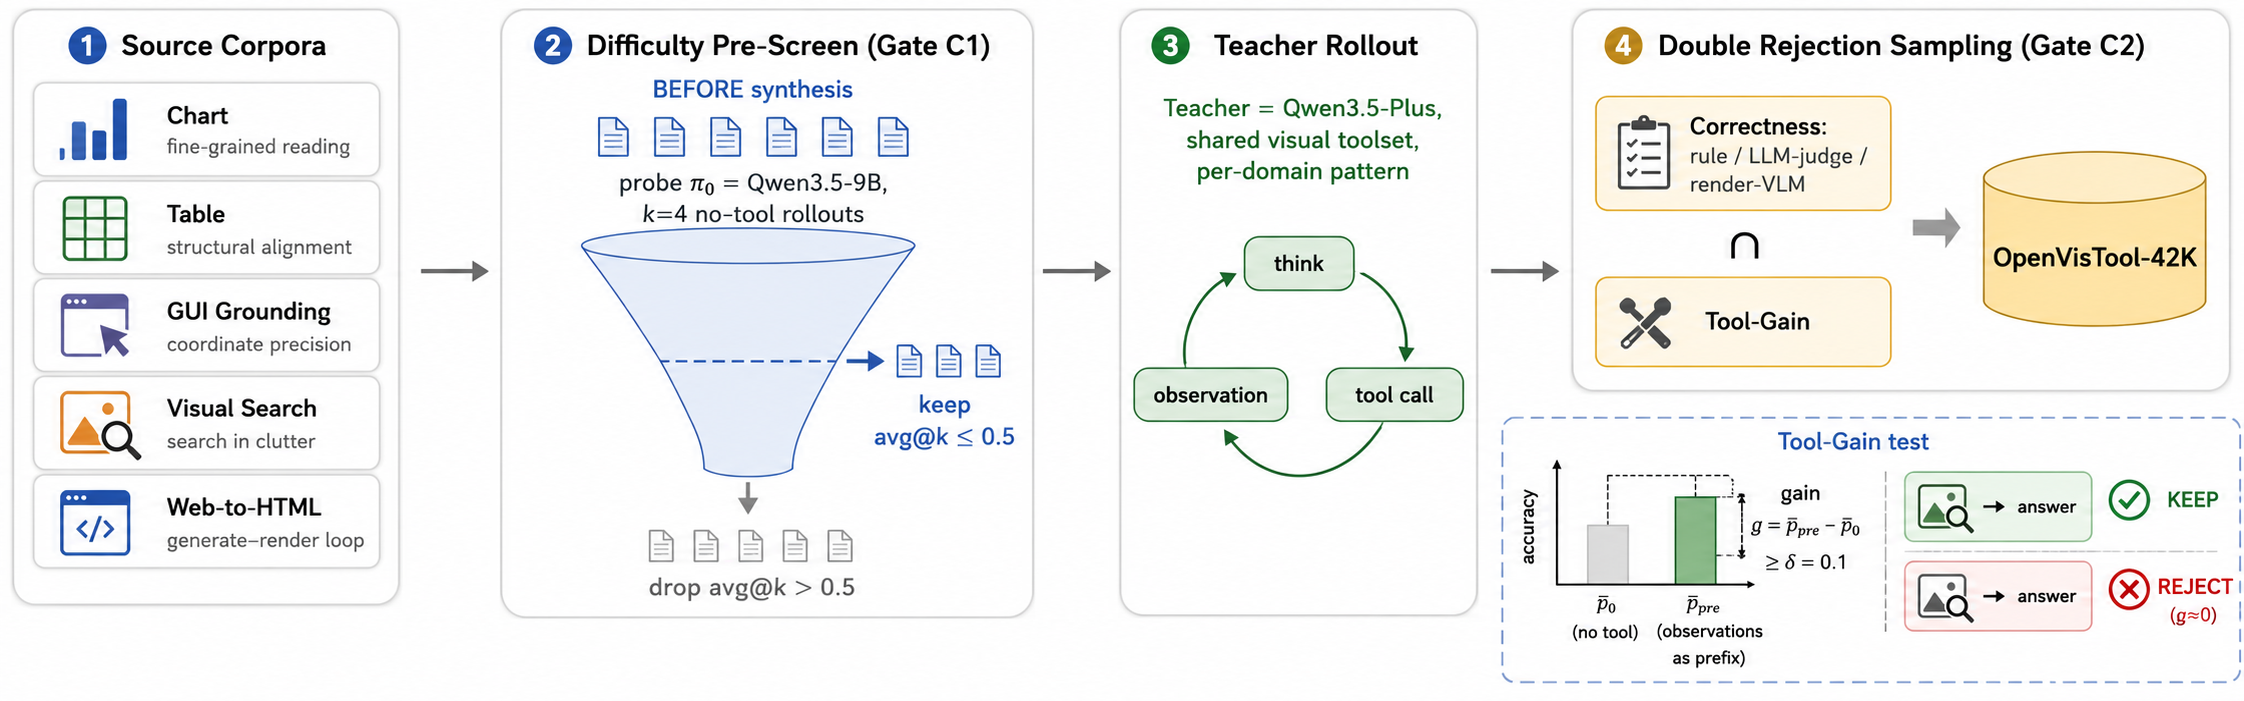
\includegraphics[width=\textwidth]{figures/synthesis_pipeline.png}
    \caption{The three-stage \method data pipeline. \textit{Difficulty Screening} selects queries that the screening model cannot reliably answer from its initial image encoding alone; \textit{Domain-Specific Tool-Use Patterns} guide the teacher to acquire evidence suited to each domain; and \textit{Supervision Verification} retains trajectories that satisfy both outcome validity and causal utility.}
    \label{fig:pipeline}
\end{figure*}

\section{\method}
\label{sec:method}

\subsection{What Makes a Trajectory Instructive?}
\label{sec:instructive-trajectory}

% 这里做一些 problem formulation，并用公式化表达
Consider a visual reasoning instance $x=(I,q,y^\star,d)$, where $I$ is the input image, $q$ is the query, $y^\star$ is the reference answer, and $d$ denotes the task domain. A candidate tool-use trajectory is represented as
\begin{equation}
\tau=\left((r_t,c_t,o_t)_{t=1}^{T},\hat{y}_{\tau}\right),
\end{equation}
where $r_t$, $c_t$, and $o_t$ denote the reasoning step, tool call, and returned observation at turn $t$, respectively, and $\hat{y}_{\tau}$ is the final answer. 
We use $O_{\tau}=\{o_1,\ldots,o_T\}$ to denote the complete set of visual observations acquired along the trajectory, and $E_d(\hat{y},y^\star)\in\{0,1\}$ to denote the domain-specific evaluator.


% An \emph{instructive trajectory} is a tool-use trajectory whose observations provide useful evidence that helps answer the query more reliably. Correctness alone does not provide this guarantee. A strong teacher may infer the answer from its internal knowledge or the original image while still making tool calls because the synthesis prompt encourages them. The resulting trace is successful but spurious: imitating it teaches the student that tools accompany a correct answer, not when their evidence is needed. Conversely, useful observations embedded in an incorrect trace would propagate flawed reasoning. We therefore retain only the intersection of outcome validity and causal utility.

A trajectory must first satisfy \textbf{Outcome Validity}:
\begin{equation}
\mathcal{V}(\tau;x)=E_d\left(\hat{y}_{\tau},y^\star\right),
\label{eq:outcome-validity}
\end{equation}
which ensures that the trajectory terminates in a correct answer.
However, correctness alone does not make it instructive: a strong teacher may infer the answer from parametric knowledge or reasoning shortcuts while still invoking tools because the synthesis prompt encourages it.
Such a trajectory is successful in outcome but spurious as supervision: it teaches that tool calls co-occur with correct answers, without establishing that the returned evidence is useful.

We therefore introduce a second condition, \textbf{Causal Utility}, to measure whether the acquired observations improve answer reliability under a controlled evidence intervention. 
Let $Y_{\pi_0}(O)$ denote the answer produced by a fixed probe model $\pi_0$ when the observation set is intervened to $O$, while the original image and query remain unchanged. 
We define
\begin{equation}
\mathcal{U}_{\pi_0}(\tau;x)=
\mathbb{E}\Big[
E_d\left(Y_{\pi_0}(O_{\tau}),y^\star\right) -
E_d\left(Y_{\pi_0}(\emptyset),y^\star\right)
\Big].
\label{eq:causal-utility}
\end{equation}
% where the expectation is taken over the stochasticity of the probe model. 
The two conditions differ only in whether $O_{\tau}$ is available; therefore, $\mathcal{U}_{\pi_0}$ captures the incremental answer utility of the observations independently of the teacher's stated reasoning.
% This utility is defined at the level of the complete observation set and relative to the fixed probe model.

A trajectory is instructive when it satisfies both conditions:
\begin{equation}
\mathcal{I}_{\delta}(\tau;x)=\mathbf{1}\left[\mathcal{V}(\tau;x)=1\;\land\;\mathcal{U}_{\pi_0}(\tau;x)\geq\delta\right].
\label{eq:instructive-criterion}
\end{equation}
% The two requirements address complementary failure modes. Outcome validity excludes trajectories that contain potentially useful observations but culminate in an incorrect answer, while causal utility excludes answer-correct trajectories whose tool observations provide no measurable benefit. Their intersection identifies demonstrations that are both reliable in outcome and grounded in externally acquired visual evidence.
Figure~\ref{fig:pipeline} turns this definition into a three-stage pipeline. 
% \textit{Difficulty Screening} selects queries that a fixed screening model cannot reliably answer from its initial image encoding alone, identifying limitations of the screening model's initial image encoding.
\textbf{Difficulty Screening} first selects queries that the probe model cannot reliably solve from the original image alone.
% \textit{Domain-Specific Tool-Use Patterns} then guide a teacher model to acquire evidence suited to each domain's visual bottleneck. 
\textbf{Domain-Specific Tool-Use Patterns} then guide a stronger teacher to acquire evidence suited to each domain's visual bottleneck. 
% Finally, \textit{Supervision Verification} tests whether the resulting trajectory satisfies outcome validity and whether its observations measurably improve the screening model's answer reliability, thereby establishing causal utility.
Finally, \textbf{Supervision Verification} evaluates outcome validity and estimates causal utility by comparing the probe model under observation-conditioned and no-observation interventions. 
Only trajectories satisfying both criteria are retained to form OpenVisTool-42K.


\subsection{Difficulty Screening}
\label{sec:data}

% We collect candidate queries from five domains---Chart, Table, GUI Grounding, Visual Search, and Web-to-HTML---that cover complementary perception bottlenecks such as dense labels, small interface elements, cluttered scenes, and layout reconstruction. We use Qwen3.5-9B \citep{qwen35blog} as a fixed screening model and run it four times per query without tools. If the screening model already solves a query reliably from its initial image encoding alone, any subsequent tool use is likely to be redundant and provides little signal about when evidence acquisition is necessary. We therefore retain a query only if the screening model succeeds on at most two attempts. Difficulty Screening removes queries already solved reliably from the initial image encoding and caches a no-tool baseline for evaluating the trajectory later. Source-specific preprocessing and corpus composition are reported in Appendix~\ref{app:datacard}.

We collect candidate instances from five domains: Chart, Table, GUI Grounding, Visual Search, and Web-to-HTML. 
Since many queries can already be solved from the original image, synthesizing tool-use trajectories for them may introduce redundant tool calls. 
We therefore screen for queries that a fixed probe model cannot reliably answer without tools.
% 这里面把 four times 换成 K 次，更加通用正式一些，实验中 K = 4
% 成功最多两次也换成了成功率不超过gamma
For each instance $x=(I,q,y^\star,d)$, we run the probe model $\pi_0$ for $K$ independent no-tool trials and compute
\begin{equation}
\bar{p}_0(x)=\frac{1}{K}\sum_{k=1}^{K}E_d\left(Y_{\pi_0}^{(k)}(\emptyset),y^\star\right).
\label{eq:no-tool-success-rate}
\end{equation}
We retain an instance if $\mathcal{C}_{\mathrm{diff}}(x)=\mathbf{1}\left[\bar{p}_0(x)\leq\gamma\right]$.
We use Qwen3.5-9B as $\pi_0$ and set $K\!=\!4, \gamma\!=\!0.5$, retaining queries answered correctly in at most two trials. 
The resulting $\bar{p}_0(x)$ is cached as the no-observation baseline for Supervision Verification in Section~\ref{sec:filtering}. 
Dataset sources and preprocessing details are provided in Appendix~\ref{app:datacard}.


\subsection{Domain-Specific Tool-Use Patterns}
\label{sec:synthesis}

% For every retained query, Qwen3.5-Plus acts as a teacher agent with a shared visual tool interface. At each turn, it reasons about what remains uncertain, invokes a tool to resolve that uncertainty, receives the resulting observation, and continues until it produces a final answer. The recorded candidate trajectory preserves this complete interaction rather than only the final response.

For each instance retained by Difficulty Screening, we use Qwen3.5-Plus as a teacher model $\pi_{\text{tea}}$ to synthesize a candidate trajectory with a shared visual toolset. 
Let $h_t$ denote the interaction history before turn $t$. 
The rollout proceeds as
\begin{equation}
\begin{aligned}
(r_t,c_t)
&\sim \pi_{\mathrm{tea}}(\cdot\mid h_t,P_d), \\
o_t
&=\operatorname{Exec}(c_t), \\
h_{t+1}
&=h_t\oplus(r_t,c_t,o_t),
\end{aligned}
\label{eq:teacher-rollout}
\end{equation}
where $P_d$ is the tool-use pattern associated with domain $d$. 
The process continues until the teacher produces a final answer, and the complete sequence of reasoning steps, tool calls, and observations is preserved.

% A generic instruction to ``use tools when helpful'' can still elicit arbitrary or decorative calls. We instead guide the teacher with domain-specific instructions derived from the visual bottleneck identified in each task family. Chart and Table trajectories align relevant regions and perform color analyais before reading or computing; GUI Grounding and Visual Search trajectories crop, localize, and verify small targets; Web-to-HTML trajectories render a draft, compare it with the reference, and revise it. The underlying tool interface remains shared across domains, so the supervision emphasizes reusable evidence-acquisition skills rather than task-specific APIs. Full instructions and representative trajectories are provided in Appendix~\ref{app:prompts} and Appendix~\ref{app:qualitative}.

A generic instruction to ``use tools when helpful'' may elicit arbitrary or decorative calls. 
We instead construct $P_d$ according to each domain's visual bottleneck: Chart trajectories localize relevant marks and inspect visual attributes before computation; Table trajectories align rows and columns before extracting values; GUI Grounding and Visual Search trajectories crop, localize, and verify small targets; and Web-to-HTML trajectories iteratively generate, render, compare, and revise a webpage.
All domains use the same underlying tool interface; only the conditions and preferred order of tool invocation differ.
Consequently, the synthesized trajectories emphasize reusable evidence-acquisition behaviors rather than domain-specific APIs. 
Full domain instructions and demos are provided in Appendices~\ref{app:prompts} and~\ref{app:qualitative}.



\subsection{Supervision Verification}
\label{sec:filtering}

% Before applying the two criteria, we remove malformed sessions, such as traces with missing observations or invalid file references. We then enforce outcome validity by rejecting trajectories whose final answer does not match the reference. The evaluator follows the output structure of each domain, using the appropriate combination of text answer matching, point-in-box evaluation, and rendered-page comparison with a VLM judge.
We first discard malformed trajectories, including sessions with missing observations, failed tool executions, or invalid file references. 
For each remaining trajectory, we verify \textbf{outcome validity} using the domain-specific evaluator $E_d$ defined in Section~\ref{sec:instructive-trajectory}.
Only trajectories satisfying $\mathcal{V}(\tau;x)=1$ in Eq.~(\ref{eq:outcome-validity}) proceed to the causal-utility test.
Depending on the domain, $E_d$ uses answer matching, point-in-box evaluation, or rendered-page comparison with a
VLM judge.



% We then test causal utility separately from the teacher's reasoning. For each trajectory that satisfies outcome validity, we extract only its tool outputs, provide them to the same fixed screening model used in Difficulty Screening, and ask the model to answer the original query four more times. A trajectory satisfies causal utility when its observation-conditioned success rate exceeds the cached no-tool baseline. Withholding the teacher's reasoning prevents the screening model from copying a solution and isolates the information supplied by the observations. Reusing the same screening model and evaluator makes the two success rates directly comparable, while using a weaker model than the teacher avoids the ceiling effect that would arise from testing the stronger teacher.


We then evaluate \textbf{causal utility}. 
For each outcome-valid trajectory, we extract its tool observations $O_\tau$ and provide them, together with the original image and query, to the same probe model $\pi_0$ used in Difficulty Screening. 
The teacher's reasoning and final answer are excluded to prevent solution leakage. 
Using $K$ independent trials, we compute
\begin{equation}
\bar{p}_{\mathrm{obs}}(x,\tau)=\frac{1}{K}\sum_{k=1}^{K}E_d\left(Y_{\pi_0}^{(k)}(O_\tau),y^\star
\right).
\label{eq:observation-success-rate}
\end{equation}
The empirical utility of the observations is defined relative
to the cached no-observation baseline:
\begin{equation}
g(x,\tau)=\bar{p}_{\mathrm{obs}}(x,\tau)-\bar{p}_0(x).
\label{eq:observation-gain}
\end{equation}
A trajectory passes Supervision Verification if
\begin{equation}
\mathcal{C}_{\mathrm{ver}}(\tau;x)=\mathbf{1}\left[\mathcal{V}(\tau;x)=1\;\land\;g(x,\tau)\geq\delta
\right].
\label{eq:supervision-verification}
\end{equation}
We use the same $K=4$ trials as in Difficulty Screening and set $\delta=0.1$. 
Reusing the same probe model and evaluator makes $\bar{p}_{\mathrm{obs}}(x,\tau)$ directly comparable with $\bar{p}_0(x)$.
Each retained sample preserves the teacher's reasoning, tool calls, observations, and final answer, enabling supervised fine-tuning to learn both when to acquire visual evidence and how to incorporate it.To measure \textbf{causal utility}, we extract only the tool observations $O_\tau$ from the trajectory and provide them to the same probe model $\pi_0$ used in Difficulty Screening.
The teacher's reasoning and final answer are excluded to prevent solution leakage. 
We sample $K$ responses and compute the observation-conditioned success rate
\begin{equation}
\bar{p}_{\mathrm{obs}}(x,\tau)
=
\frac{1}{K}
\sum_{k=1}^{K}
E_d\left(
Y_{\pi_0}^{(k)}(O_\tau),y^\star
\right).
\label{eq:observation-success-rate}
\end{equation}
We then estimate the utility of the observations relative to
the cached no-observation baseline:
\begin{equation}
g(x,\tau)
=
\bar{p}_{\mathrm{obs}}(x,\tau)-\bar{p}_0(x).
\label{eq:observation-gain}
\end{equation}
Let $\mathcal{M}(\tau)$ indicate that a trajectory is
well-formed. The supervision-verification rule is
\begin{equation}
\mathcal{C}_{\mathrm{ver}}(\tau;x)
=
\mathbf{1}
\left[
\begin{aligned}
&\mathcal{M}(\tau)=1
\;\land\;
\mathcal{V}(\tau;x)=1 \\
&{}\land\;
g(x,\tau)\geq\delta
\end{aligned}
\right].
\label{eq:supervision-verification}
\end{equation}
We use $K=4$ and $\delta=0.1$. Since the empirical success
rates change in increments of $0.25$, this criterion requires
the observations to produce at least one additional correct
response.
Detailed rollout settings and filter hyperparameters are provided in Appendices~\ref{app:pipeline} and \ref{app:hyperparams}.



% The trajectories that satisfy both outcome validity and causal utility form \dataset. Each retained sample preserves the reasoning, tool arguments, observations, and final answer, allowing supervised fine-tuning to teach both when to seek evidence and how to incorporate it. Detailed rollout settings and filter hyperparameters are provided in Appendix~\ref{app:pipeline} and Appendix~\ref{app:hyperparams}.Detailed rollout settings and filter hyperparameters are provided in 
Appendix~\ref{app:pipeline} and Appendix~\ref{app:hyperparams}.